\documentclass{beamer}

% To have the citation lists ordered by number.
\usepackage[utf8]{inputenc}
\usepackage{graphicx}
\usepackage[tight,TABTOPCAP]{subfigure}
\usepackage{amsmath}
\usepackage{amssymb}
\usepackage{amsfonts}
\usepackage{url}
\usepackage{xspace}

\usepackage{hyperref}

\usepackage{tikz}
\usetikzlibrary{calc}
\usetikzlibrary{shapes.symbols}
\usetikzlibrary{shapes}
\usepackage{color}


\mode<presentation>
{
  \usetheme{Warsaw}
  %\usetheme{Frankfurt}
  % or ...

  %\setbeamercovered{transparent}
  % or whatever (possibly just delete it)
  %\setbeamertemplate{footline}[frame number]
  \useoutertheme{mysplit}
}
% Remove the navigation bar
\setbeamertemplate{navigation symbols}{}

\graphicspath{{./figs/}}

\title[Automating Separation Logic using SMT]{Automating Separation Logic using SMT}

\iffalse
\AtBeginSection[]
{
  \begin{frame}<beamer>
    \frametitle{Outline}
    \tableofcontents[currentsection,hideothersubsections]
  \end{frame}
}
\fi

\author[Damien Zufferey]{
  Ruzica Piskac \and
  Thomas Wies \and
  \emph{Damien Zufferey}
}

\institute{ MPI-SWS \hspace{10mm} NYU \hspace{10mm} IST Austria }
\date{CAV, July 17 2013, Saint Petersburg}


\newcommand{\letin}[2]{\textrm{let } #1 = #2 \textrm{ in}}
\newcommand{\set}[1]{\{#1\}}
\newcommand{\pset}[2]{\set{\,#1\mid#2\,}}
\newcommand{\pto}{\rightharpoonup}

\newcommand{\nullobj}{\m{null}}

\newcommand{\rank}{\m{rank}}
\newcommand{\mkframe}{\mathit{Frame}}
\newcommand{\ep}{\mathit{ep}}

\newcommand{\awrite}{\mathit{wr}}
\newcommand{\ato}[3]{#1 \stackrel{#3}{\rightsquigarrow} #2}
\newcommand{\atoto}[3]{#1 \stackrel{#3}{\leftrightsquigarrow} #2}
\newcommand{\aread}{\mathit{rd}}
\newcommand{\adiff}{\mathit{diff}}

\newcommand{\fldread}{\mathit{fieldRead}}
\newcommand{\fldwrite}{\mathit{fieldWrite}}
\newcommand{\blank}{\mathord{\color{black!33}\bullet}}%
\newcommand{\reachsymf}{\blank \xrightarrow{\blank \setminus \blank} \blank}
\newcommand{\reachsym}{\xrightarrow{\edge \setminus}}

\newcommand{\fwrite}[3]{#1[#2 := #3]}
\newcommand{\fread}[2]{#2.#1}
\newcommand{\reachf}[3]{#2 \xrightarrow{#1} #3}
\newcommand{\reach}[2]{\reachf{\edge}{#1}{#2}}
\newcommand{\reachModel}[3]{#1 \rightarrow^{#3} #2}
\newcommand{\creachf}[4]{#2 \xrightarrow{#1 \setminus #4} #3}
\newcommand{\creach}[3]{\creachf{\edge}{#1}{#2}{#3}}
\newcommand{\cset}[2]{\{#1.\,#2\}}
\newcommand{\creachModel}[4]{#1 \mathrel{\vphantom{\xrightarrow{\edge \setminus #3}}
  \smash{\xrightarrow{\edge \setminus #3}}
  \vphantom{\to}^{#4}} #2}
\newcommand{\edge}{h}
%\newcommand{\join}[2]{\joinsym(#1,#2)}
\newcommand{\nil}{\mathsf{nil}}
\newcommand{\univset}{\mathcal{U}}

\newcommand{\Btwn}{\mathit{Btwn}}
\newcommand{\BtwnWO}{\mathit{BtwnWO}}
\newcommand{\m}[1]{\mathsf{#1}}
\newcommand{\mi}[1]{\textit{#1}}

\newcommand{\emp}{\mathsf{emp}}
\newcommand{\liste}[2]{\m{ls}({#1},{#2})}
\newcommand{\listen}[3]{\m{ls}^{#3}({#1},{#2})}
\newcommand{\JoshLogicSimple}{\textsf{SLL}\xspace}
\newcommand{\JoshLogic}{$\JoshLogicSimple\mathbb{B}$\xspace}
\newcommand{\JoshLogicFull}{\JoshLogic(Boolean combinations of separation logic formulas for linked lists)}
\newcommand{\LRJQ}{\textsf{GRASS}\xspace}
\newcommand{\lrjq}{\mathsf{GS}}
\newcommand{\lrjqaxioms}{\mathcal{K}_{\lrjq}}
\newcommand{\lrjqmodels}{\mods_{\lrjq}}
\newcommand{\lrjqtheory}{\theory_{\lrjq}}
\newcommand{\lrjqinterp}{\theory_{\lrjq,\vars}}
\newcommand{\lrjqsig}{\sig_{\lrjq}}
\newcommand{\lrjqentails}{\models_\lrjq}
\newcommand{\graph}{\mathsf{G}}
\newcommand{\graphtheory}{\theory_\graph}
\newcommand{\sets}{\mathsf{S}}
\newcommand{\settheory}{\theory_\sets}
\newcommand{\reduce}{\mathit{reduce}}

\newcommand{\Tool}{\textsc{GRASShopper}\xspace}
\newcommand{\zthree}{\textsc{Z3}\xspace}

\newcommand{\hsucc}{\mathit{succ}}

%-----------------------------------------------------
% Theories, Models, etc
\newcommand{\alg}{\mathcal{A}}%{\alpha}
\newcommand{\oalg}{\mathcal{B}}%{\alpha}
\newcommand{\va}{\beta}
\newcommand{\sig}{\Sigma}
\newcommand{\sorts}{S}
\newcommand{\funs}{\Omega}
\newcommand{\vars}{\mathcal{X}}
\newcommand{\consts}{\Gamma}
\newcommand{\preds}{\Pi}
\newcommand{\dompreds}{\mathcal{D}}

\newcommand{\support}[1]{[#1]}
\newcommand{\substruct}{\subseteq}
\newcommand{\supstruct}{\supseteq}

\newcommand{\theory}{\mathcal{T}}
\newcommand{\theoryeuf}{\theory_{\m{EUF}}}
\newcommand{\Models}{\m{Mod}}
\newcommand{\mods}{\mathcal{M}}


\newcommand{\fldsort}{\m{field}}
\newcommand{\boolsort}{\m{bool}}
\newcommand{\nodesort}{\m{node}}
\newcommand{\setsort}{\m{set}}

\newcommand{\cardsym}{\m{card}}
\newcommand{\card}[1]{\cardsym({#1})}



\newcommand{\Terms}[1]{\m{Terms}(#1)}

%-----------------------------------------------------
% Local theory extensions

\newcommand{\theoryext}{\mathcal{K}}
\newcommand{\sigext}{\sig_e}
\newcommand{\funext}{\funs_e}
\newcommand{\st}{\m{st}}
\newcommand{\Loc}{($\m{Loc}^\Psi$)\xspace}
\newcommand{\pmodels}{\m{PMod}}

\newcommand{\weld}{W}


% -------------------------------------------------------------
% Logical ops
\newcommand{\mimplies}{\mathop{\Rightarrow}}
\newcommand{\miff}{\mathop{\Leftrightarrow}}

\newcommand{\fcom}[2]{{#1}^{[#2]}}

\newcommand{\meq}{\mathord{=}}


%-------------------------------

\def\pointsto{\mapsto}
\def\ls{\mathsf{ls}}

\newcommand{\strfun}{\mathit{str}}
\newcommand{\str}[2]{\strfun_{#1}(#2)}
\def\tr{\mathit{tr}}
\def\itr{\mathit{tr}^{-1}}
\def\itrfull{\mathit{Tr}^{-1}}
\def\ftrfull{\mathit{Trf}}
\newcommand{\trfull}[2]{\mathit{Tr}_{#2}(#1)}
\def\disjoint{\mathit{dj}}
\def\idisjoint{\mathit{idj}}
\def\structure{\mathit{st}}
\def\footprint{\mathit{fp}}
\def\tightness{\mathit{tc}}

\newcommand{\SL}{{\mathsf{SL}}}
\newcommand{\slforms}{\mathcal{H}}
\newcommand{\tightentails}{\models_\SL}
%\newcommand{\entailsLolli}{\models_l}
\newcommand{\tightmodels}[3]{{#1},{#2} \models_\SL {#3}}
\newcommand{\tightmodelsStandard}[1]{\tightmodels{\alg}{X}{#1}}
\newcommand{\intumodels}[4]{{#1},{#2},{#3} \models_i {#4}}
\newcommand{\intumodelsStandard}[1]{\intumodels{\alg}{\beta}{D}{#1}}

\newcommand{\sel}{\mathsf{sel}}
\newcommand{\upd}{\mathsf{upd}}

\newcommand{\new}[1]{\textbf{new}(#1)}
\newcommand{\dispose}[1]{\textbf{dispose}(#1)}
\newcommand{\assert}{\textbf{assert}}
\newcommand{\assume}{\textbf{assume}}
\newcommand{\steprel}[1]{\stackrel{#1}{\leadsto}}
\newcommand{\alloc}{\mathsf{Alloc}}
\newcommand{\error}{\mathsf{fail}}
\renewcommand{\wp}{\mathsf{wp}}
\newcommand{\ite}[3]{\mathrm{if}\; #1 \; \mathrm{then} \; #2 \; \mathrm{else} \; #3}

\newcommand{\var}{\mathit{var}}

\lstdefinelanguage{SPL}{
  morekeywords={struct,if,else,returns,procedure,requires,ensures,:=,var,new,old,free,implicit,modifies,
                call,locals,assume,assert,choose,havoc,ghost,predicate,function},
  deletekeywords={union,int},
  lineskip=-0.1em,
  numbers=none,
%  stepnumber=2,    
%  firstnumber=1,
%  numberfirstline=true,
%  numbers=none,
  numberstyle=\tiny,
  basicstyle=\scriptsize\sffamily,
  columns=flexible,
  morecomment=*[s][\textsl]{/*:}{*/},
  morecomment=*[l][\textsl]{//:},
  mathescape=true,
}
\lstset{language=SPL}


%-------------------------------------------------------------------------
\begin{document}

% Title
\frame[plain]{\titlepage}

\iffalse
\begin{frame}
  \frametitle{Motivation}
  Separation logic (SL) succinctly express invariants of heap configurations.

  \vspace{1ex}

  Good features:\\
  \mbox{} ~~ Spatial conjunction (*),\\
  \mbox{} ~~ Inductive spatial predicates (list, tree, etc.),\\
  \mbox{} ~~ Frame rule.

  \vspace{1ex}

  Not so good features:\\
  Specialized provers for decidable fragments means that extension and combination with other solvers/theories is not straightforward.

\end{frame}

\begin{frame}
  \frametitle{Example}
  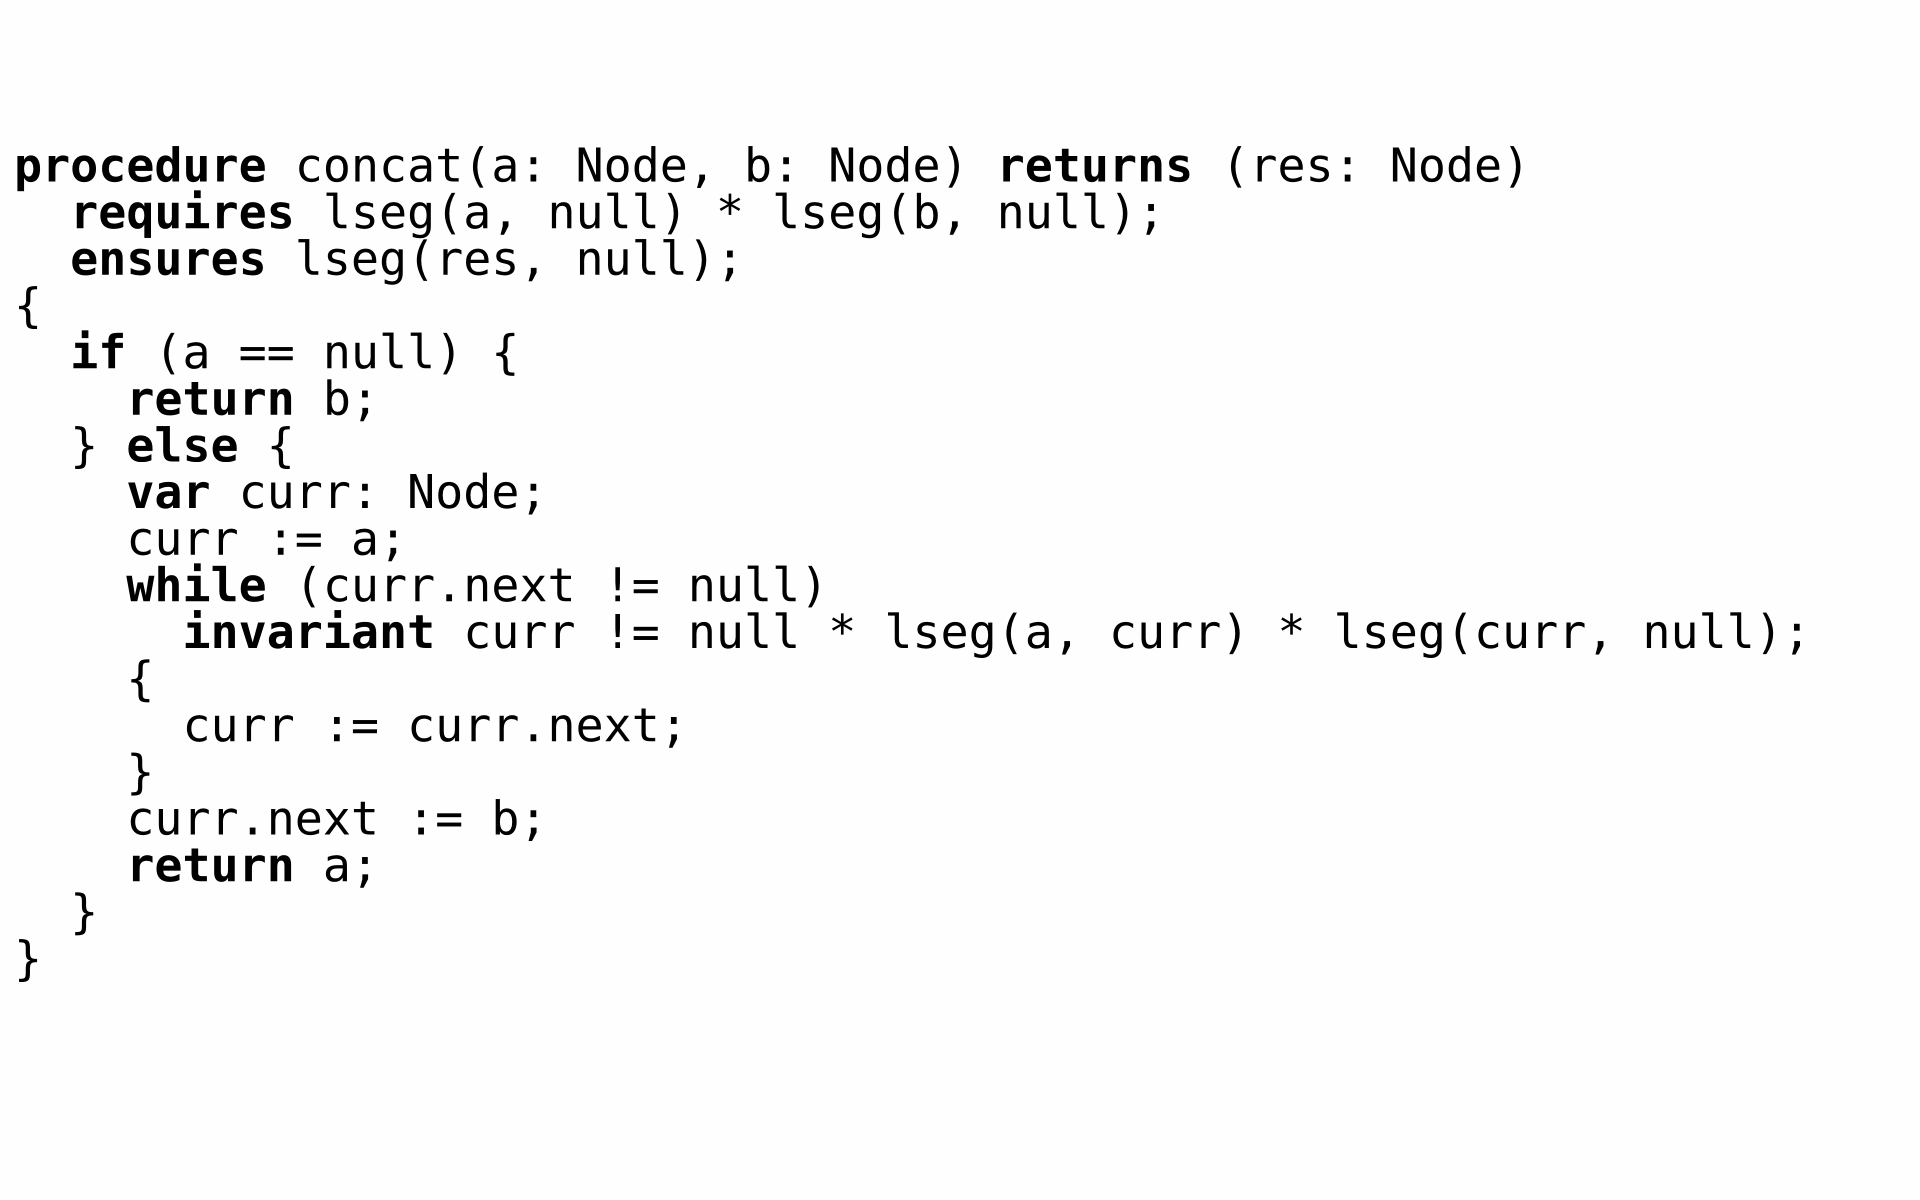
\includegraphics[scale=0.17]{resources/concat.png}
\end{frame}
\fi

\begin{frame}
  \frametitle{Motivation}
  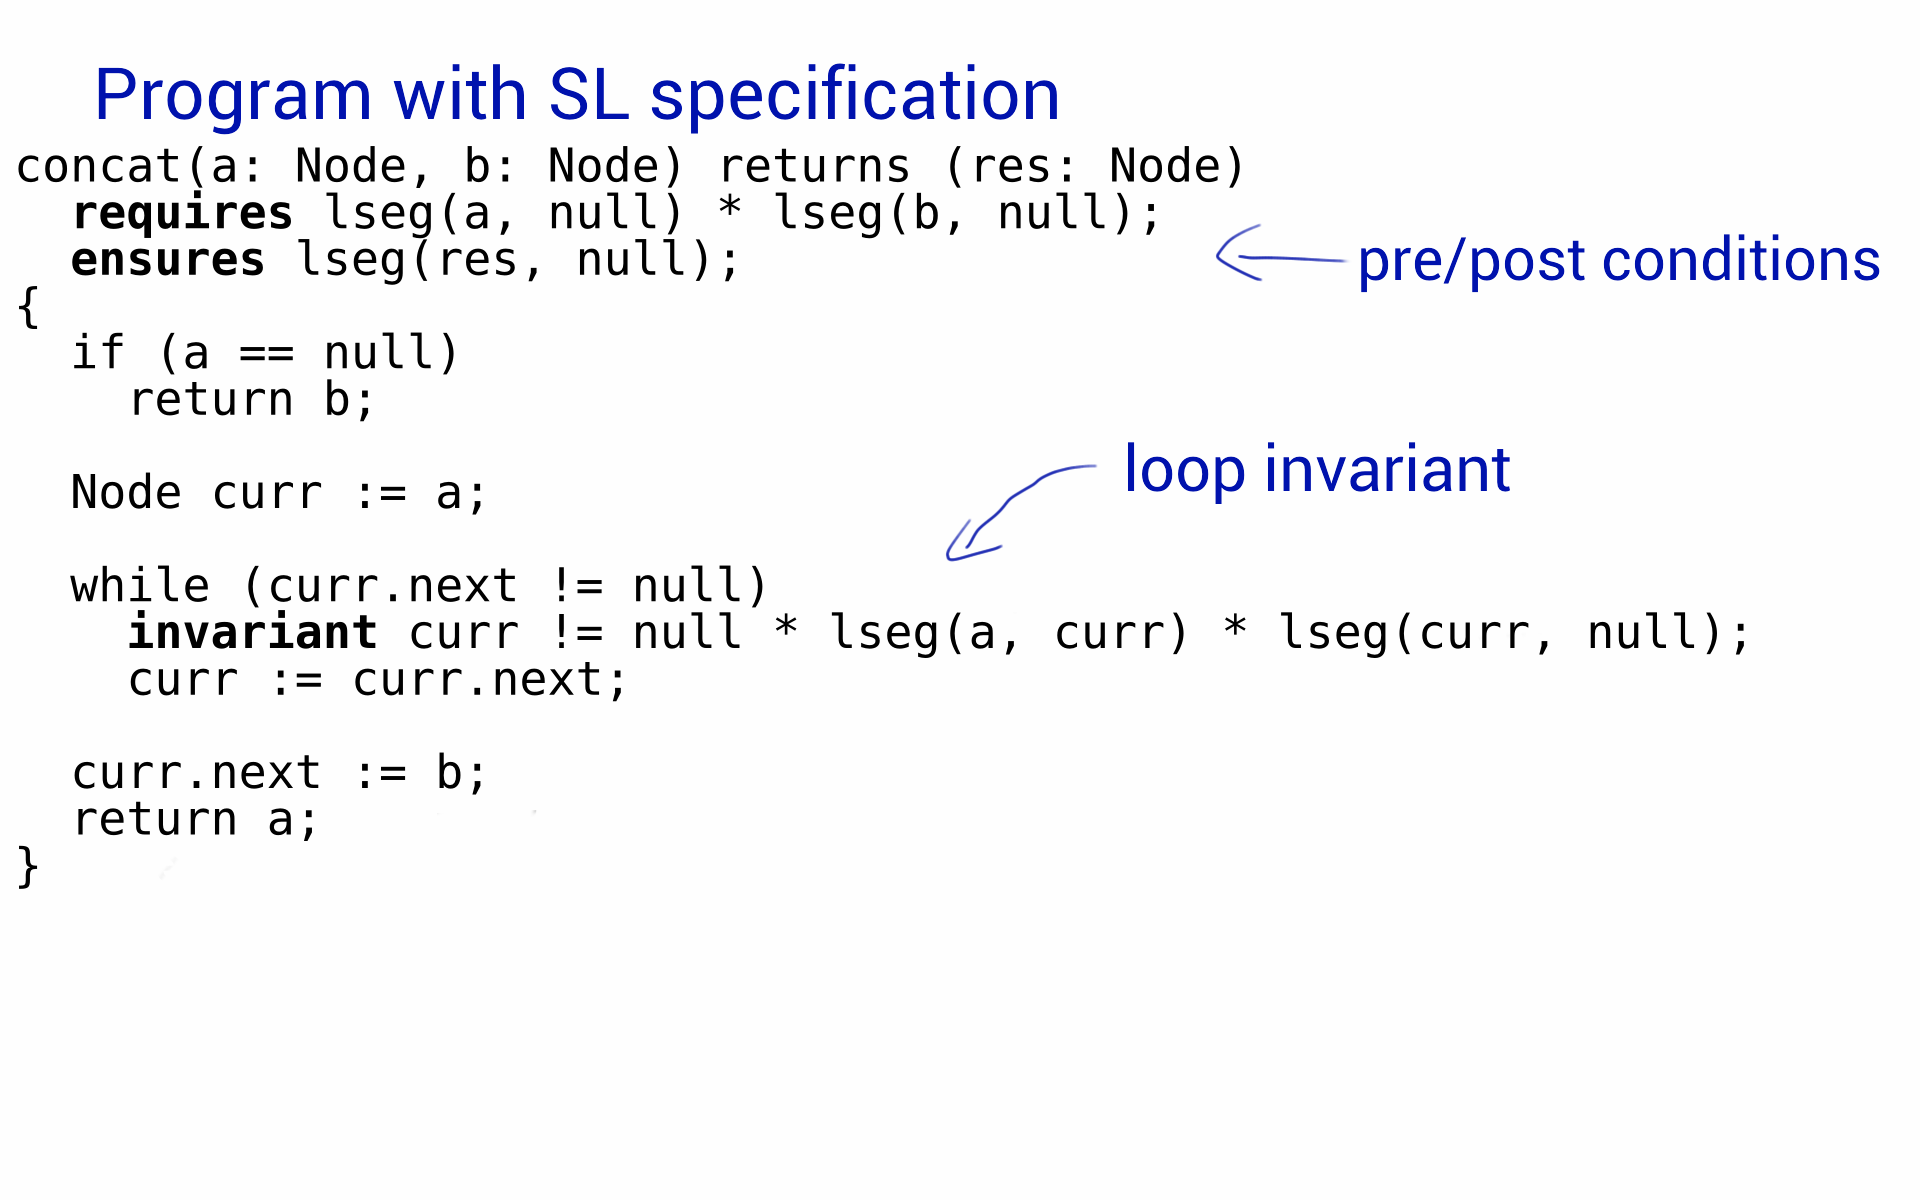
\includegraphics[scale=0.17]{resources/spec.png}
\end{frame}

\begin{frame}
  \frametitle{Motivation}
  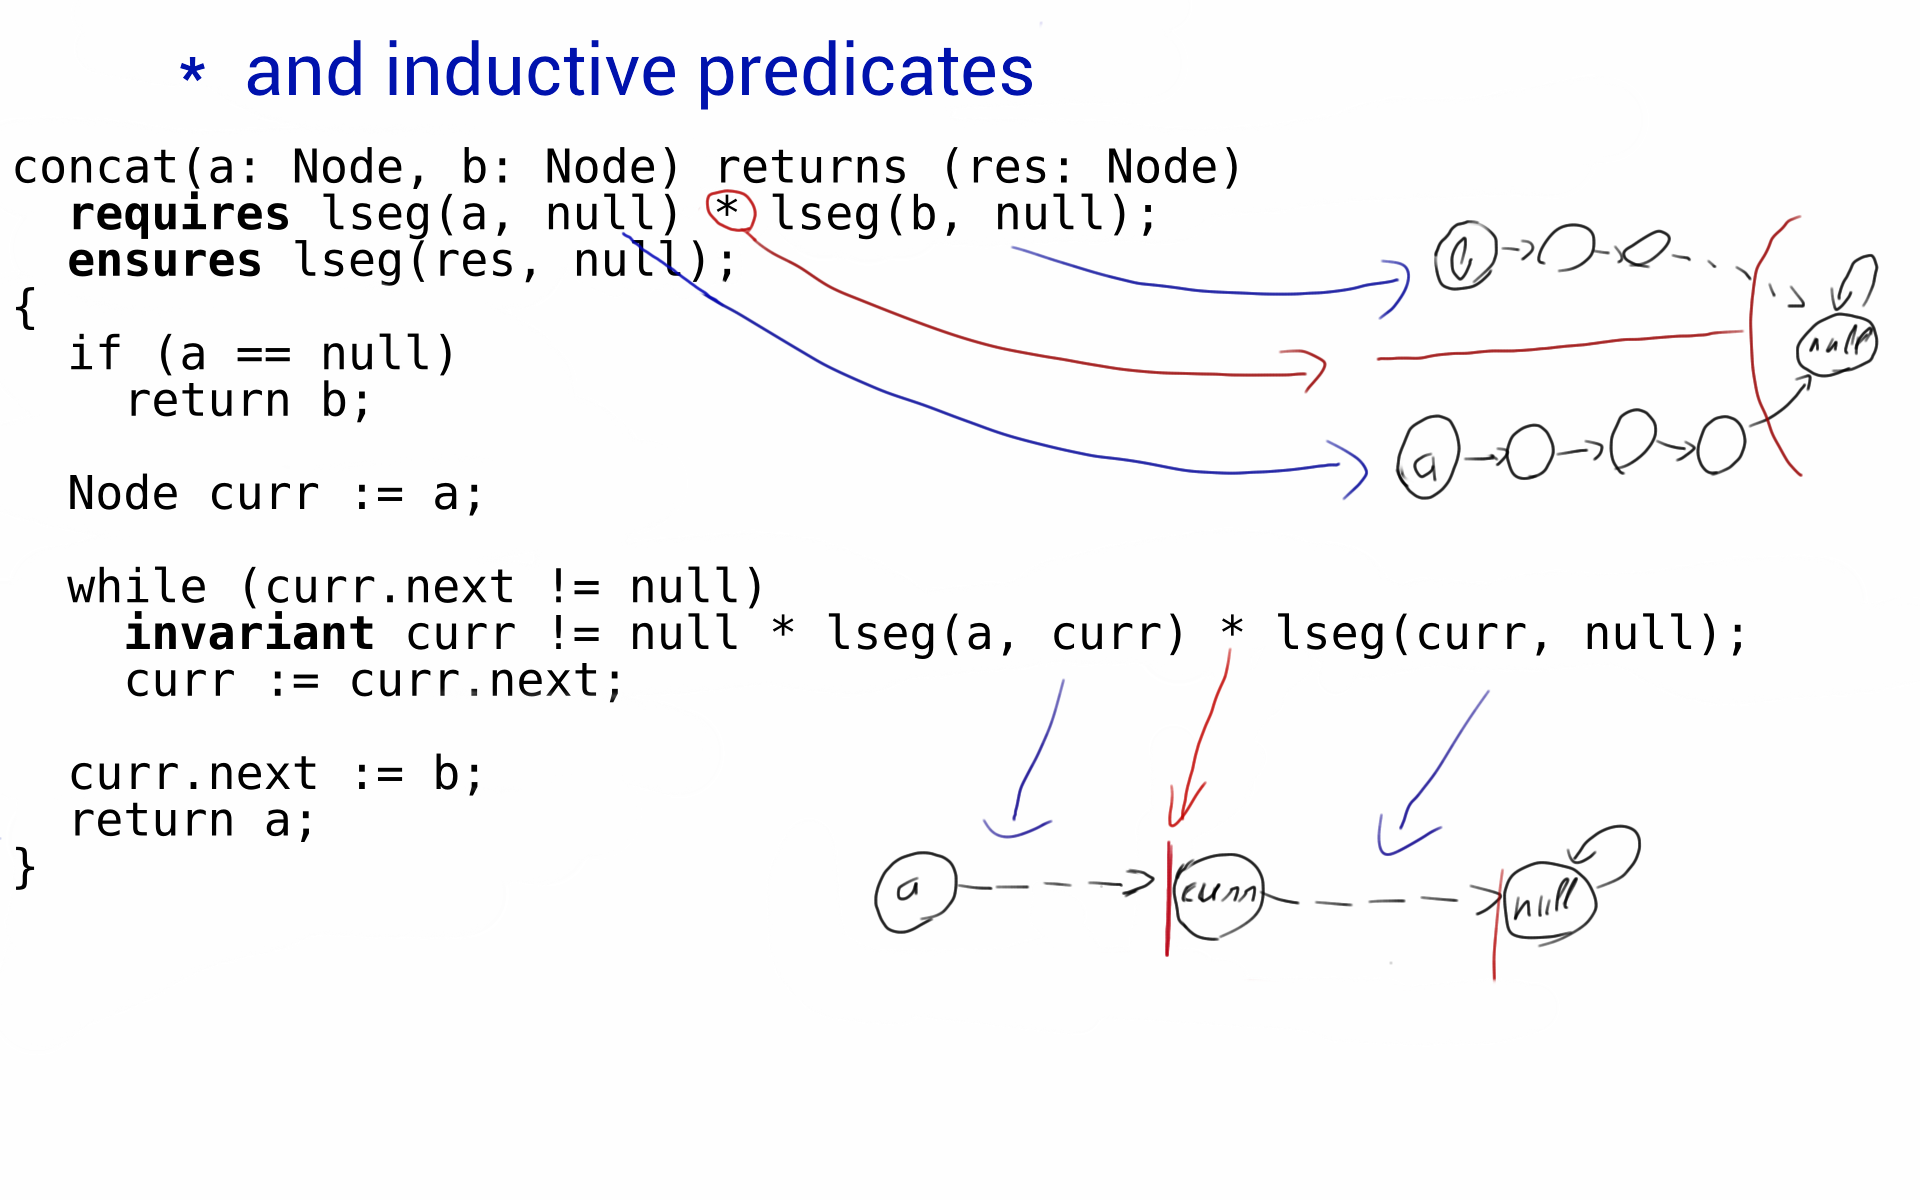
\includegraphics[scale=0.17]{resources/star.png}
\end{frame}

\begin{frame}
  \frametitle{Motivation}
  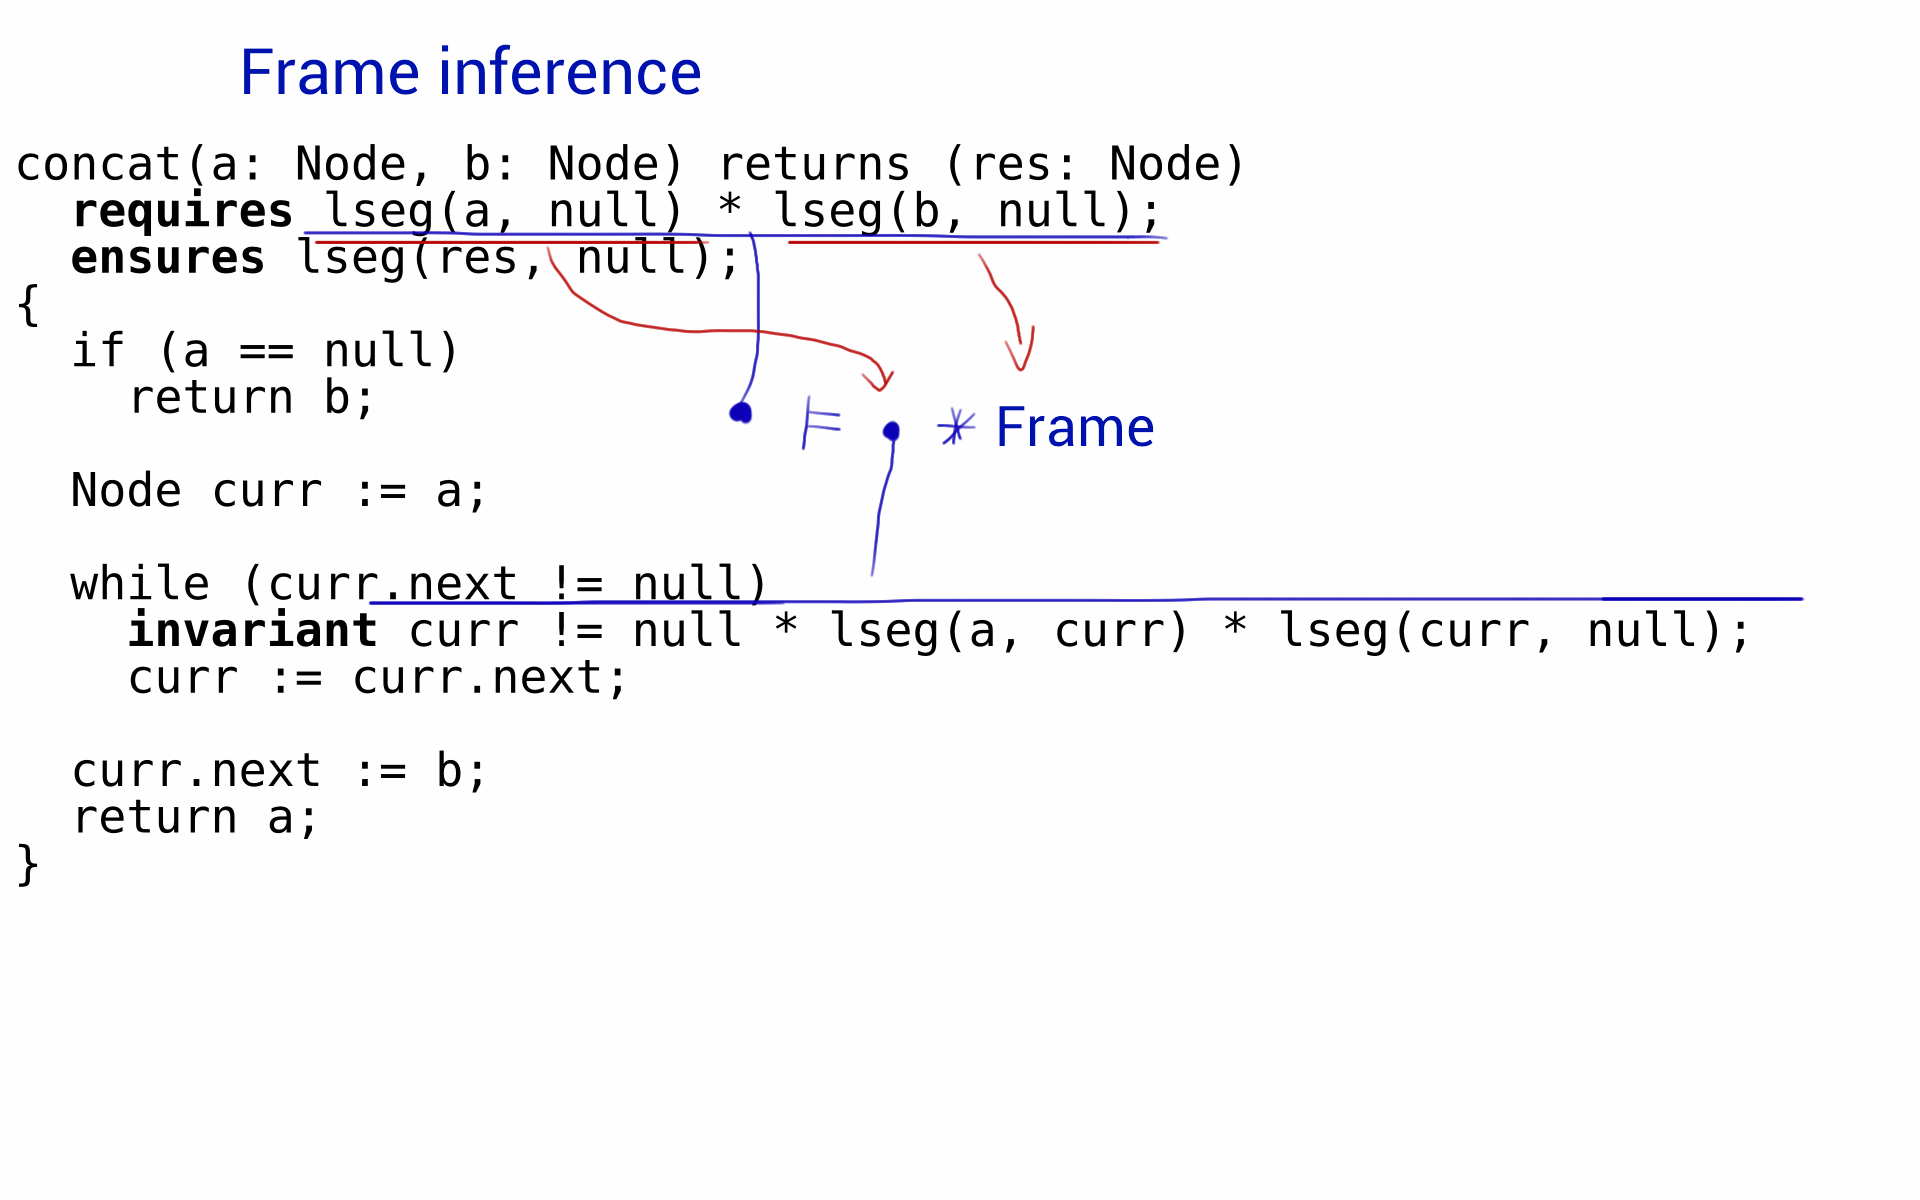
\includegraphics[scale=0.17]{resources/frame.png}
\end{frame}

\begin{frame}
  \frametitle{Motivation}
  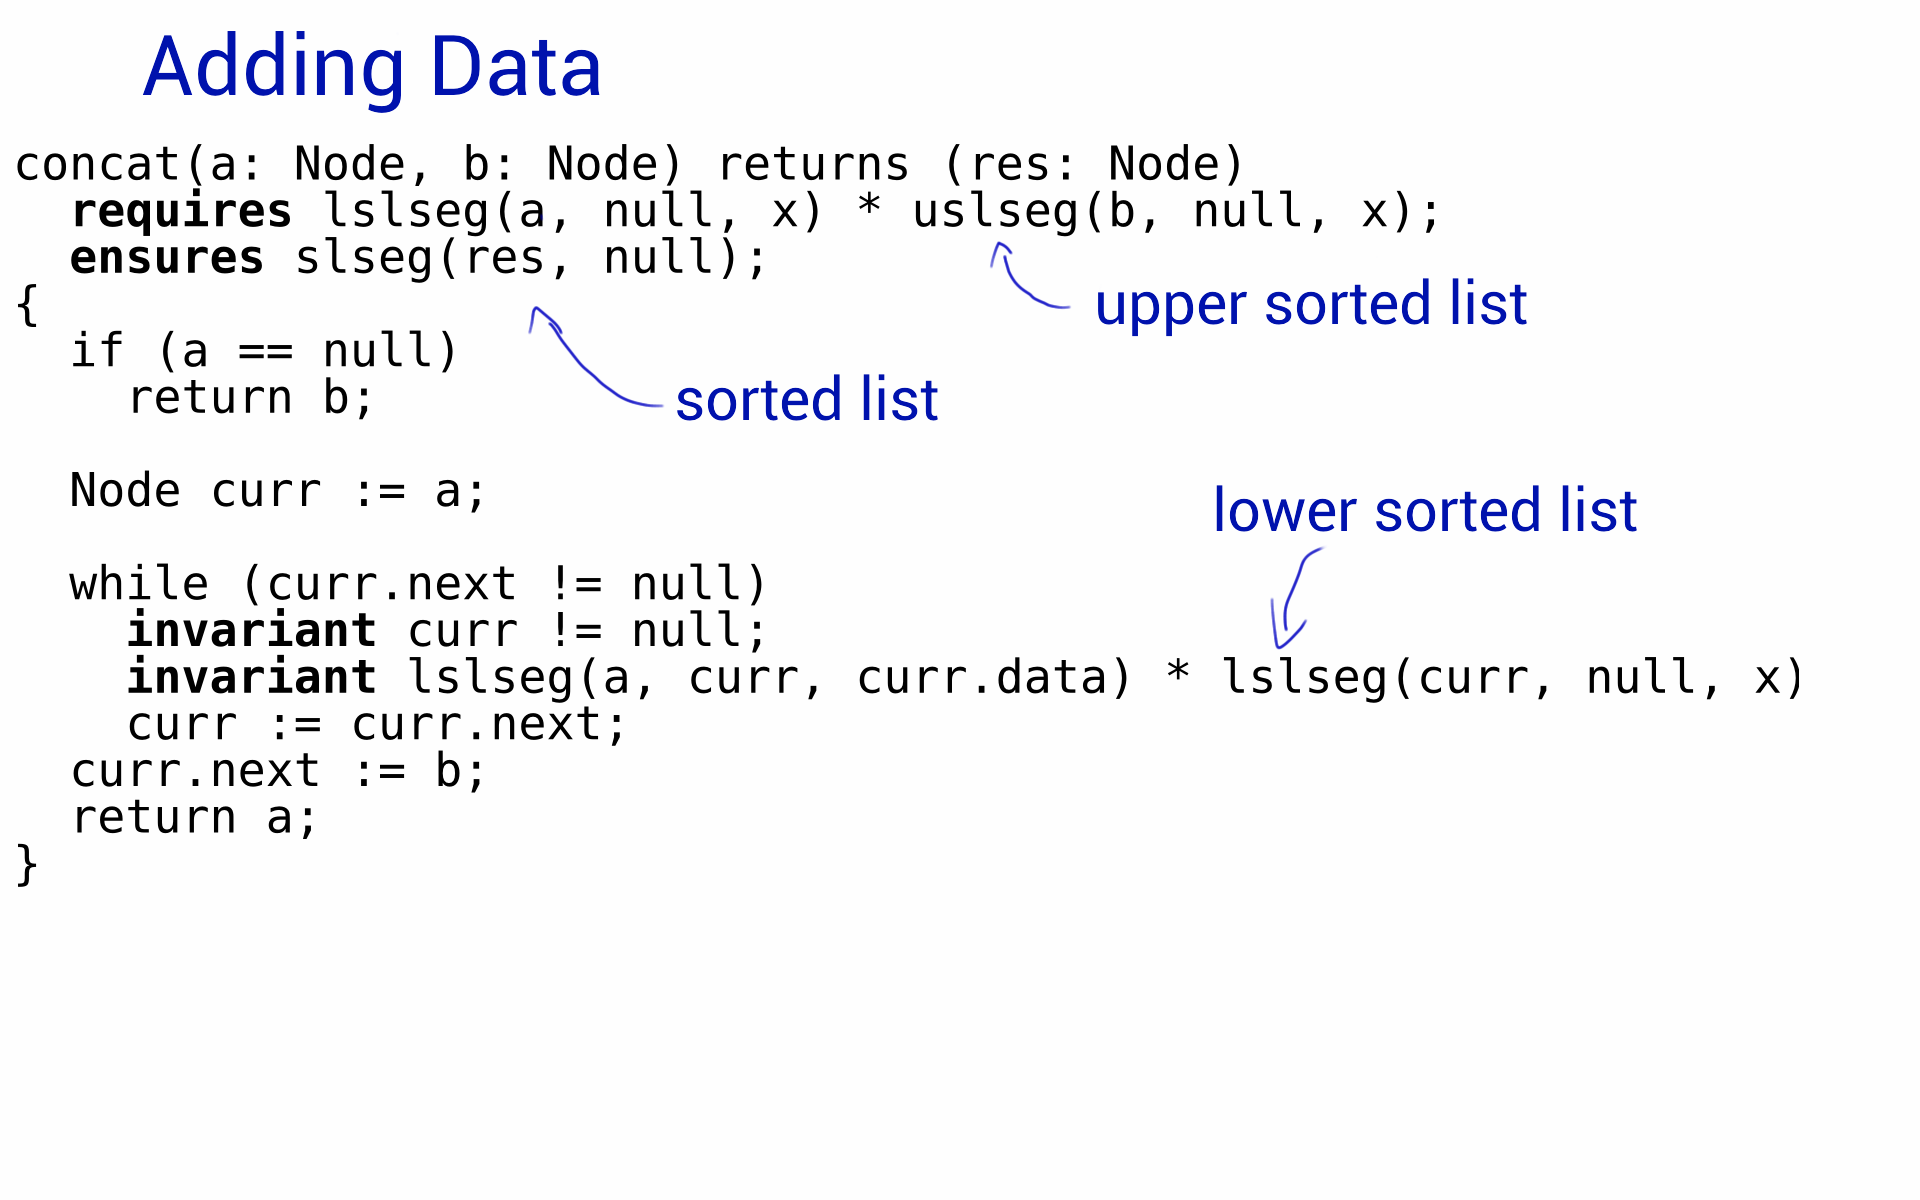
\includegraphics[scale=0.17]{resources/sorted.png}
\end{frame}

\begin{frame}
  \frametitle{Our work}

  \begin{itemize}
  \item Reduce a decidable fragment of SL to a decidable FO theory.
  \item Combining SL with other theories.
  \item Satisfiability, entailment, frame inference, and abduction problems for SL using SMT solvers.
  \item Implemented in the GRASShopper tool.
  \end{itemize}

\end{frame}

\section{$\text{SLL}\mathbb{B}$ $\leftrightarrow$ GRASS}

\subsection{$\text{SLL}\mathbb{B}$}

\begin{frame}
  \frametitle{Decidable SL fragment: \JoshLogic}

\JoshLogicSimple (separation logic formulas for linked lists) introduced in \cite{BerdineETAL04DecidableFragmentSeparationLogic}.

\vspace{2ex}

\JoshLogicSimple
\begin{equation*}
  \Sigma ::= x = y \mid x \neq y \mid x \mapsto y \mid \liste{x}{y} \mid \Sigma * \Sigma
\end{equation*}
%$x,y \in \vars$

\vspace{2ex}

With extend \JoshLogicSimple to \JoshLogic by adding boolean connective on top:
\begin{equation*}
  H ::= \Sigma \mid \neg H \mid H \land H
\end{equation*}

\end{frame}

\iffalse
\begin{frame}
  \frametitle{Semantics of \JoshLogic (1)}

$\tightmodelsStandard{H}$ \\[2ex]
$\mathcal{A}$: heap interpretation (total) \\
$X$: is the footprint of the formula (also interpreted in $\mathcal{A}$) \\[4ex]

We use the tight interpretation of SL, i.e. the heap contains only the nodes specified by $H$.

\end{frame}
\fi

\begin{frame}
  \frametitle{Semantics of \JoshLogic (1)}
  $\Sigma ::= \alert{x = y} \mid \alert{x \neq y} \mid \alert{x \mapsto y} \mid \liste{x}{y} \mid H_1 * H_2$

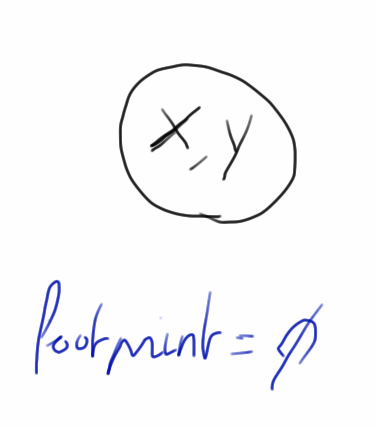
\includegraphics[scale=0.20]{resources/sl_eq.png}
\hfill
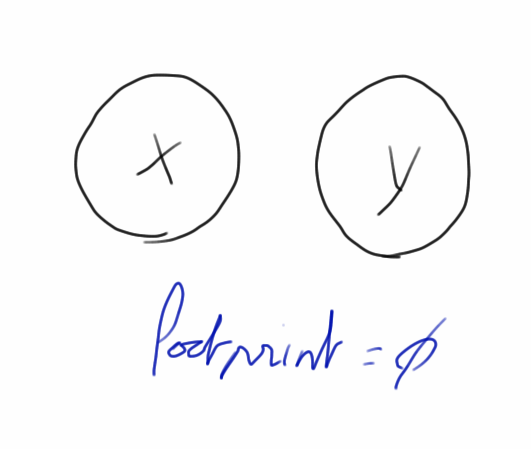
\includegraphics[scale=0.20]{resources/sl_neq.png}

\begin{center}
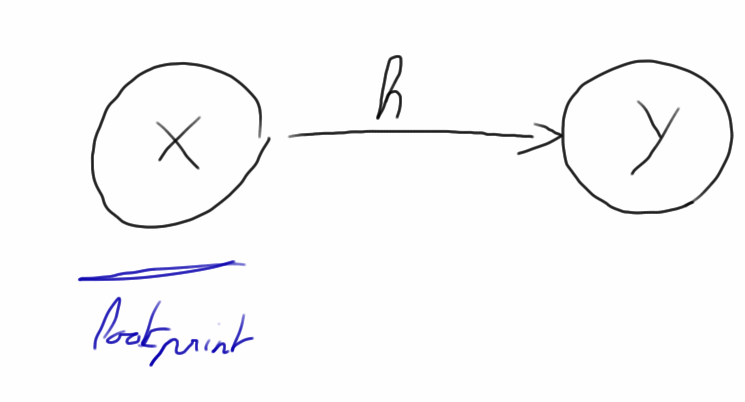
\includegraphics[scale=0.20]{resources/sl_pts.png}
\end{center}

\end{frame}

\begin{frame}
  \frametitle{Semantics of \JoshLogic (2)}
  $\Sigma ::= x = y \mid x \neq y \mid x \mapsto y \mid \liste{x}{y} \mid \alert{H_1 * H_2}$

\begin{center}
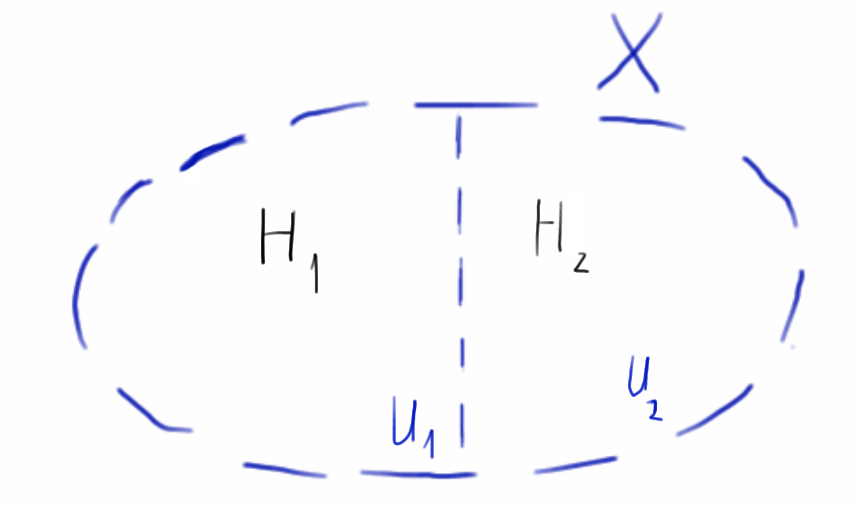
\includegraphics[scale=0.20]{resources/sl_star.png}
\end{center}

important: $ \exists U_1, U_2 $

\end{frame}

\begin{frame}
  \frametitle{Semantics of \JoshLogic (3)}
  $\Sigma ::= x = y \mid x \neq y \mid x \mapsto y \mid \alert{\liste{x}{y}} \mid H_1 * H_2$

\begin{center}
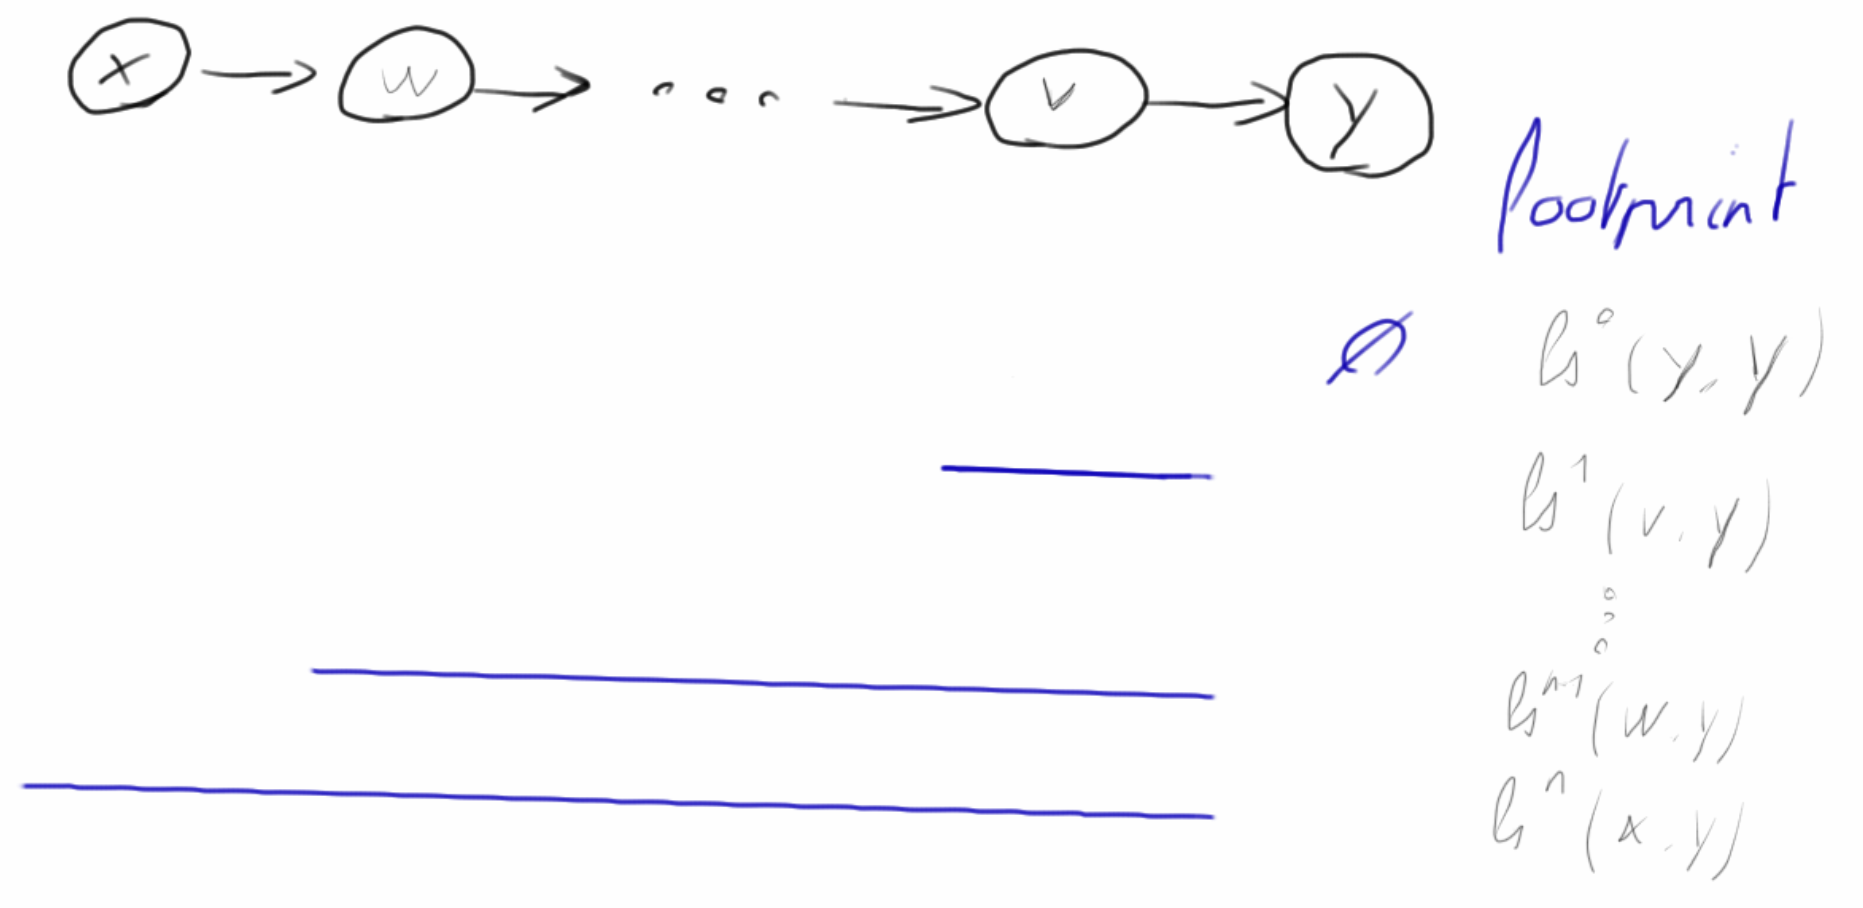
\includegraphics[scale=0.14]{resources/sl_ls.png}
\end{center}

\end{frame}

\iffalse
\begin{frame}
  \frametitle{Semantics of \JoshLogic (3)}

\begin{align*}
 &\tightmodelsStandard{H_1 \land H_2}&
\text{iff  }&  \tightmodelsStandard{H_1} \text{ and } \tightmodelsStandard{H_2} \\[3ex]
 &\tightmodelsStandard{\neg H}&
\text{iff  }&  \text{not } \tightmodelsStandard{H}
\end{align*}

\end{frame}
\fi

\subsection{GRASS}

\begin{frame}
  \frametitle{\JoshLogic $\quad \rightarrow \quad$ \LRJQ}

  Translate \JoshLogic to a decidable FO theory.\\[1ex]

  Requirements:
  \begin{itemize}
  \item easy automation with SMT solvers
  \item well-behaved under theory combination
  \item no increase in complexity
  \end{itemize}  

  \vspace{1ex}

  \LRJQ: combination of two theories
  \begin{itemize}
  \item structure: \emph{functional graph reachability} ($\graphtheory$)\\ to encode the shape of the heap (pointers)
  \item footprint: \emph{stratified sets} ($\settheory$)\\ to encode the part of the heap used by a formula
  \end{itemize}  
  

\end{frame}


\begin{frame}
  \frametitle{\LRJQ: graph reachability and stratified sets}

\begin{equation*}
\begin{array}{rcl}
  & & \text{graph reachability} \\
  T & ::= & x \mid \edge(T) \\
  A & ::= & T = T \mid \creach{T}{T}{T} \\
  R & ::= & A \mid \neg R \mid R \land R \mid R \lor R \\
   & & \\
  & & \text{stratified sets} \\
  S & ::= & X \mid \emptyset \mid S \setminus S \mid S \cap S \mid S \cup S \mid \cset{x}{R} \quad \text{$x$ not below $h$ in $R$} \\
  B & ::= & S = S \mid T \in S \\
   & & \\
  & & \text{top level boolean combination} \\
  F & ::= & A \mid B \mid \lnot F \mid F \land F \mid F \lor F 
  \end{array} 
\end{equation*}

\end{frame}

\iffalse
\begin{frame}
  \frametitle{$\graphtheory$: theory of function graphs}

  \begin{minipage}{.5\linewidth}
  Function graph:\\
  \mbox{}\ one outgoing edge per node\\[1ex]
  Reachability:\\
  \mbox{}\ reflexive-transitive closure
  \end{minipage}
  \hfill
  \begin{minipage}{.4\linewidth}
  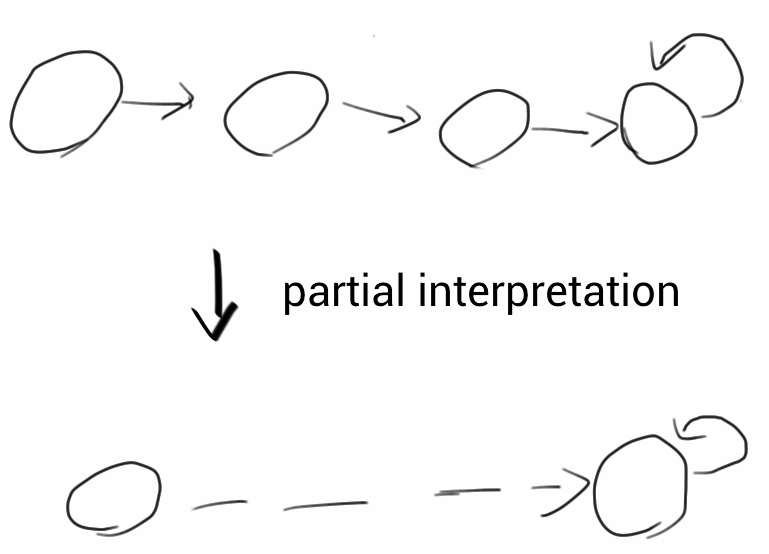
\includegraphics[scale=0.15]{resources/partial.png}
  \end{minipage}

\end{frame}
\fi

\begin{frame}
  \frametitle{$\graphtheory$: theory of function graphs}
  
  $\creach{t_1}{t_2}{t_3}$ is true if there exists a path in the graph of $h$ that connects $t_1$ and $t_2$ without going through $t_3$.
  
  \vspace{1ex}

  \begin{center}
  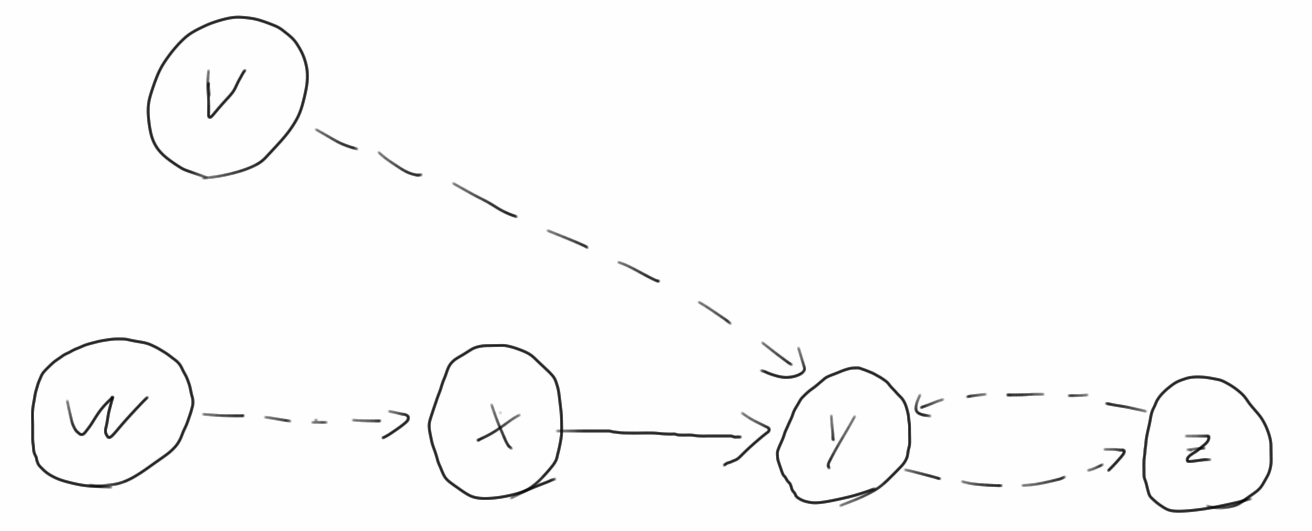
\includegraphics[scale=0.18]{resources/reach_ex.png}
  \end{center}

  \begin{minipage}{.45\linewidth}
  $\reach{w}{w}$ (reflexivity)\\[1ex]
  $\reach{x}{y}$ (induced by $h$)
  \end{minipage}
  \begin{minipage}{.45\linewidth}
  $\neg\reach{v}{w}$ (no path)\\[1ex]
  $\neg\creach{x}{z}{y}$ ($y$ is before $z$)
  \end{minipage}\\[1ex]
  $\Btwn(w,z) = \{y. \creach{w}{y}{z} \land z \neq y\} = \{ w,x,y \}$

\end{frame}

\subsection{$\text{SLL}\mathbb{B}$ $\rightarrow$ GRASS}

\begin{frame}
  \frametitle{\JoshLogic $\quad \rightarrow \quad$ \LRJQ (1)}

  Usual way of translating SL to FO:
  \begin{itemize}
  \item structure: $\graphtheory$ to encode the shape of the heap (pointers)
  \item footprint: $\settheory$ to encode the part of the heap used by a formula
  \end{itemize}

  \vspace{2ex}
  
  Negation (entailment check, frame) $\Rightarrow$ more complicated 
  \begin{itemize}
  \item structure: uses $\graphtheory$ and $\settheory$ to encode the shape of the heap (pointers) and disjointness
  \item set definition: uses $\settheory$ for keep track of the sets that will make the footprint
  \end{itemize}
  
\end{frame}

\begin{frame}
  \frametitle{\JoshLogic $\ \rightarrow \ $ \LRJQ : interesting cases}
  \begin{align*}
    \trfull{H}{X} = {} & \letin{(F,G)}{\tr_X(H)} \; F \land G \\
    {} & \text{$F$ is the structure} \\
    {} & \text{$G$ is the set definitions.} \\[1ex]
    %
    \tr_{X}(\ls(x,y)) = {} & (\reach{x}{y},\;  X = \Btwn(x,y)) \\[1ex]
    %
    \tr_{X}(\Sigma_1 * \Sigma_2) = {} &
    \text{let } \text{$Y_1,Y_2 \in \vars$ fresh } \\
    & \text{ and } (F_1,G_1) = \tr_{Y_1}(\Sigma_1) \\
    & \text{ and } (F_2,G_2) = \tr_{Y_2}(\Sigma_2)\\
    & \text{in } (F_1 \land F_2 \land Y_1\!\cap\!Y_2\!=\!\emptyset,\;     X\!=\!Y_1\!\cup\!Y_2 \land G_1 \land G_2)\\[1ex]
    %
    \tr_X(\neg H) = {} &
    \letin{(F,G)}{\tr_{X}(H)} \; (\neg F,\; G)
  \end{align*}
  
  
\end{frame}

\iffalse
\begin{frame}
  \frametitle{\JoshLogic $\ \rightarrow \ $ \LRJQ : ~ $*$ or below}
  \begin{align*}
    \str{Y}{x = y} = {} & (x = y,\; Y = \emptyset) \\
    %
    \str{Y}{x \neq y} = {} & (x \neq y,\; Y = \emptyset) \\[1ex]
    %
    \str{Y}{x \mapsto y} = {} & (\edge(x)=y,\; Y = \{x\})\\[1ex]
    %
    \str{Y}{\ls(x,y)} = {} & (\reach{x}{y},\;  Y = \Btwn(x,y)) \\[1ex]
    %
    \str{Y}{\Sigma_1 * \Sigma_2} = {} &
    \text{let } \text{$Y_1,Y_2 \in \vars$ fresh } \\
    & \text{ and } (F_1,G_1) = \tr_{Y_1}(\Sigma_1) \\
    & \text{ and } (F_2,G_2) = \tr_{Y_2}(\Sigma_2)\\
    & \text{in } (F_1 \land F_2 \land Y_1\!\cap\!Y_2\!=\!\emptyset,\;     Y\!=\!Y_1\!\cup\!Y_2 \land G_1 \land G_2)\\
  \end{align*}
\end{frame}

\begin{frame}
  \frametitle{\JoshLogic $\ \rightarrow \ $ \LRJQ : ~ boolean structure}
  \begin{align*}
    \tr_X(\Sigma) = {} & \text{let } \text{$Y \in \vars$ fresh and } (F,G) = \str{Y}{\Sigma} \\
    & \text{ in }(F \land X\!=\!Y,\; G)\\[1ex]
    %
    \tr_X(\neg H) = {} &
    \letin{(F,G)}{\tr_{X}(H)} \; (\neg F,\; G)\\[1ex]
    %
    \tr_X(H_1\!\land\!H_2) = {} &
    \text{let } (F_1,G_1) = \tr_X(H_1) \text{ and }
    (F_2,G_2) = \tr_X(H_2) \\
    & \text{in }(F_1 \land F_2,\; G_1 \land G_2)\\[1ex]
    %
    \trfull{H}{X} = {} & \letin{(F,G)}{\tr_X(H)} \; F \land G
  \end{align*}%
\end{frame}
\fi

\begin{frame}
  \frametitle{Example: without negation}
a non-empty acyclic list segment from $x$ to $z$
\[ x \neq z \textcolor{red}{*} x \mapsto y * \textcolor{blue}{\liste{y}{z}} \]

translate to
\[
\begin{array}{l}
x \neq z \land
\edge(x)=y \land
\textcolor{blue}{\reach{y}{z}} \land
\textcolor{red}{Y_2\!\cap\!Y_3 = \emptyset} \land
Y_4\!\cap\!Y_5 = \emptyset \land
X = Y_1 \land {} \\
\textcolor{red}{Y_1\!=\!Y_2\!\cup\!Y_3} \land
Y_2\!=\!\emptyset \land
Y_3\!=\!Y_4\!\cup\!Y_5 \land %{} \\
Y_4\!=\!\{x\} \land
\textcolor{blue}{Y_5\!=\!\Btwn(y,z)}
\end{array}
\]
\end{frame}

\begin{frame}[2]
  \frametitle{Example: with negation}
a non-empty acyclic list segment from $x$ to $z$
\[ \alert<2>{\neg} ( \alert<1>{x \neq z* x \mapsto y * \liste{y}{z}} ) \]

\alt<1>{ignoring the negation (same as before):}{with negation}
\[
\begin{array}{l}
\text{structure \visible<2>{(\alert{negated})}}\\
\alt<1>{
x \neq z \land \edge(x)=y \land \reach{y}{z} \land
Y_2\!\cap\!Y_3 = \emptyset \land
Y_4\!\cap\!Y_5 = \emptyset \land
X = Y_1
}{
x = z \lor \edge(x) \neq y \lor \neg\reach{y}{z} \lor
Y_2\!\cap\!Y_3 \neq \emptyset \lor
Y_4\!\cap\!Y_5 \neq \emptyset \lor
X \neq Y_1
}\\[1ex]

\text{set definitions \visible<2>{(\alert{unchanged})}}\\
Y_1\!=\!Y_2\!\cup\!Y_3 \land
Y_2\!=\!\emptyset \land
Y_3\!=\!Y_4\!\cup\!Y_5 \land %{} \\
Y_4\!=\!\{x\} \land
Y_5\!=\!\Btwn(y,z)
\end{array}
\]
\end{frame}

\begin{frame}
  \frametitle{Why is that correct ?}
    
Translation: $\trfull{H}{X} = \ \letin{(F,G)}{\tr_X(H)} \; F \land G$

\vspace{2ex}

the auxiliary variables \alert{$Y_i$} (in $G$) \alert{are existentially quantified}

\vspace{1ex}

below negation, the existential quantifiers should become universal

\vspace{2ex}

the $Y_i$ are defined as finite unions of set comprehensions\\
$\rightarrow$ \alert{satisfiable in any given heap interpretation $\alg$}

\vspace{2ex}

Due to the precise semantics of \JoshLogic\\
$\rightarrow$ \alert{exists exactly one assignment of the $Y_i$} that makes $G$ true in $\alg$

\vspace{1ex}

$\exists Y_1,\dots,Y_n.\, F \land G$ \ \  and\\
$\forall Y_1,\dots,Y_n.\, G \Rightarrow F$ \ are equivalent. 

\end{frame}

\begin{frame}
  \frametitle{Where are we now ?}
  With the \JoshLogic to \LRJQ translation we can
  \begin{itemize}
  \item Check for satisfiability
  \item Check entailment (reduces to satisfiability of $H_1 \land \neg H_2$)
  \end{itemize}

  \vspace{3ex}

  We also have \LRJQ to \JoshLogic to
  \begin{itemize}
  \item compute $F$ in $A \tightentails B*F$ (frame)
  \item compute $F$ in $A*F \tightentails B$ (antiframe)
  \end{itemize}
  The details are in the paper.
  
\end{frame}

\iffalse
\begin{frame}
  \frametitle{Frame inference}
\begin{enumerate}
\item Checking whether there is a frame
\begin{align*}
\mathit{NoFrame}(A,B) & = \trfull{A}{X} \land \ftrfull_X(\neg B)
\end{align*}
where $X \in \vars$ and $\ftrfull$ is like $\mathit{Tr}$, except that the constraints $X=Y$ in the case for $\tr_X(\Sigma)$ are replaced by $Y \subseteq X$.\\[3ex]
  
\item Constructing the frame
\begin{align*}
\mathit{Frame}_Z(A,B) & = \trfull{A}{X} \land \trfull{B}{Y} \land Z\!=\!X \setminus Y  
\end{align*}
The set variable $Z$ describes the footprint of the frame.
\end{enumerate}

\end{frame}

\begin{frame}
  \frametitle{\LRJQ $\ \rightarrow \ $ \JoshLogic}

  Requirements:
  \begin{itemize}
  \item a \LRJQ formula $F$ (some restrictions)
  \item a model generating SMT solver (e.g. \zthree),
  \end{itemize}

  Steps:
  \begin{itemize}
  \item get for all the partial interpretations that satisfy $F$
  \item for all a partial interpretation:
  \begin{itemize}
  \item construct $\hsucc: \nodesort \pto \nodesort$ (closest successor in the model)
  \item extract the ${} = {}$, ${} \neq {}$ part from the interpretation
  \item lift the interpretation to SL using $h$ and $\hsucc$.
  \end{itemize}
  \end{itemize}
  where $\hsucc$ is the closest successor node in the partial interpretation

\end{frame}

\begin{frame}
  \frametitle{\LRJQ $\ \rightarrow \ $ \JoshLogic: example }

$\ldots$\\
assume($\ls(x,z)$);\\
if ($x \neq z$)\\
\mbox{} ~~~~ free\_head($x$); //frame with precondition $x\mapsto y$\\
$\ldots$\\

\vspace{1ex}

\LRJQ:
{\small $x \neq z \land \reach{x}{z} \land \edge(x)\!=\!y \land  X\!=\!\Btwn(x,z) \land Y\!=\!\set{x} \land Z\!=\!X \setminus Y$}
  
\pause{}
\vspace{.5ex}

Partial interpretations:
\begin{minipage}{0.5\linewidth}
  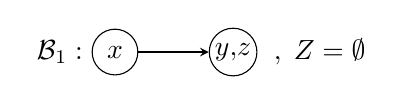
\begin{tikzpicture}
  \node (a) at (-.7,0) {$\oalg_1:$};
  \node[draw,circle] (x) at (0,0) {$x$};
  \node[draw,circle,inner sep=1pt] (y) at (1.5,0) {$y,\!z$};
  \node (Z) at (2.6,0) {$, \; Z = \emptyset$};
  % \node (yd) at (2,-.5) {\tiny$\emptyset$};
  \path[-stealth] (x) edge (y);
  \end{tikzpicture}\\[.5ex]
  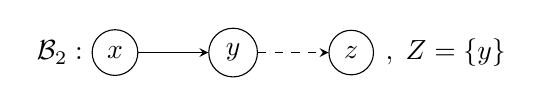
\begin{tikzpicture}
  \node (a1) at (4,0) {$\oalg_2:$};
  \node[draw,circle] (x1) at (4.7,0) {$x$};
  \node (Z1) at (8.9,0) {$, \; Z = \set{y}$};
  \node[draw,circle] (y1) at (6.2,0) {$y$};
  \node[draw,circle] (z1) at (7.7,0) {$z$};
  \path[-stealth] (x1) edge (y1);
  \path[-stealth,dashed] (y1) edge (z1);
  \end{tikzpicture}
\end{minipage}

\pause{}
\vspace{1ex}
$\itr_Z(\oalg_1)= x\!\neq\!z * x\!\neq\!y * y\!=\!z$\\
$\itr_Z(\oalg_2) = x\!\neq\!z * x\!\neq\!y * y\!\neq\!z * \ls(y,z)$\\[1ex]
$\itrfull_Z(F) = \itr_Z(\oalg_1) \lor \itr_Z(\oalg_2) \equiv x\!\neq\!z * x\!\neq\!y * \ls(y,z)$.

\end{frame}
\fi

\begin{frame}
  \frametitle{Combination with other theories and extensions}
  \begin{itemize}
  \item The theories $\graphtheory$ and $\settheory$ are stably infinite with respect to sort $\nodesort$. (Nelson-Oppen)

  \item Data: we can add data and constraints (see paper for details). 

%{\scriptsize
%$\str{Y}{\mathsf{sls}(x,y)} = (\reachf{\mathit{h}}{x}{y} \land \forall z, w \in Y.\, \reachf{\mathit{h}}{z}{w} \Rightarrow \mathit{d}(z)\! \leq\! \mathit{d}(w), \; Y\!=\!\Btwn(x,y))$
%}

  \item More pointers: we can extend the signature with $\fldsort$ and uses $\reachsymf$ with different fields.
  We can the also do read and write on the fields (array theory).

  \item More complex data structures, e.g. doubly linked lists

%{\scriptsize
%$
%\begin{array}{l}
%\str{Y}{\mathsf{dlls}(x,a,y,b)} =
% ( \begin{array}[t]{l}
%  \reachf{n}{x}{y} \land (x\!=\!y \land a\!=\!b \lor   p(x)\!=\!a \land n(b)\!=\!y \land b \in Y) \land {} \\
%\forall z \in Y.\, n(z) \in Y \Rightarrow p(n(z))\!=\!z, \;
%Y\!=\!\Btwn(x,y) \; )
%\end{array}
%\end{array}
%$
%}

  \end{itemize}
\end{frame}

\section{\Tool}

\begin{frame}
  \frametitle{Experimental results}

Implementation: \Tool available at \url{https://cs.nyu.edu/wies/software/grasshopper/}

\begin{table}[t]%{l}{5cm}
{\tiny
\centering
%\begin{minipage}{.\linewidth}
\renewcommand{\tabcolsep}{0.14cm}
\begin{tabular}{|l|c|c|c|c|c|c|c|c||l|c|c|c|c|c|c|c|c|}
\hline
program & \multicolumn{2}{|c|}{sl} & \multicolumn{2}{|c|}{dl} & \multicolumn{2}{|c|}{rec sl} & \multicolumn{2}{|c||}{sls} & 

program & \multicolumn{2}{|c|}{sl}  & \multicolumn{2}{|c|}{dl} & \multicolumn{2}{|c|}{rec sl} & \multicolumn{2}{|c|}{sls}
\\

\cline{2-9}
\cline{11-18}
%\hline

& \# & t & \# & t & \# & t & \# & t &
& \# & t & \# & t & \# & t & \# & t \\

\hline
%\hline

concat & 4 & 0.1 & 5 & 1.3 & 6 & 0.6 & 5 & 0.2 & 
insert & 6 & 0.2 & 5 & 1.5 & 5 & 0.2 & 6 & 0.4 \\

%\hline

copy    & 4 & 0.2 & 4 & 3.9 & 6 & 0.8 & 7 & 3.5 & 
reverse & 4 & 0.1 & 4 & 0.5 & 6 & 0.2 & 4 & 0.2 \\

%\hline

filter & 7 & 0.6 & 5 & 1.1 & 8 & 0.4 & 5 & 1.1 & 
remove & 8 & 0.2 & 8 & 0.8 & 7 & 0.2 & 7 & 0.5 \\

%\hline

free     & 5 & 0.1 & 5 & 0.3 & 4 & 0.1 & 5 & 0.1 & 
traverse & 4 & 0.1 & 5 & 0.3 & 3 & 0.1 & 4 & 0.2 \\

\cline{2-7}
\cline{11-16}

%\hline

\multicolumn{7}{|l|}{insertion sort} & 10 & 0.7 &
\multicolumn{7}{|l|}{double all} & 7 & 2.2\\

\multicolumn{7}{|l|}{merge sort} & 25 & 24 &
\multicolumn{7}{|l|}{pairwise sum} & 10 & 20 \\
\hline
\end{tabular}
}
\end{table}

\begin{minipage}{.5\linewidth}
\begin{description}
\item[sl] singly-linked list\\ (loop or recursion)
\item[dl] doubly-linked list
\item[sls] sorted lists
\end{description}
\end{minipage}
\begin{minipage}{.45\linewidth}
\begin{description}
\item[\#] number of VCs
\item[t] total time in s.
\end{description}
\end{minipage}
\end{frame}

\begin{frame}
  \frametitle{Conclusion}

  \begin{itemize}
  \item Reduce a decidable fragment of SL to a decidable FO theory.
  \item Combining SL with other theories.
  \item Satisfiability, entailment, frame inference, and abduction problems for SL using SMT solvers.
  \item Implemented in the GRASShopper tool.
  \end{itemize}

\end{frame}

\begin{frame}
  \frametitle{Related work}
{\small
  \begin{itemize}
  \item Most prominent decidable fragments of SL: linked lists~\cite{BerdineETAL04DecidableFragmentSeparationLogic}, decidable in polynomial time~\cite{CooketALFragmentSepLog} (graph-based).

\item SL $\rightarrow$ FO: \cite{Calcagno05fromseparation} (no inductive predicate) and~\cite{bobot12icfem} (not a decidable fragment).
%Neither of these approaches considers frame inference, abduction, or theory combination.
%More recently and concurrently to us, they have also considered the problem of theory combination~\cite{PerezR13}. The authors of~\cite{DBLP:conf/atva/BouajjaniDES12} describe another hybrid approach in which an SL decision procedure for entailment is extended to enable reasoning about quantified constraints on data. However, \cite{DBLP:conf/atva/BouajjaniDES12} does not address theory combination in general. Also, neither~\cite{DBLP:conf/pldi/PerezR11} nor~\cite{DBLP:conf/atva/BouajjaniDES12} consider frame inference or abduction.

\item Alternatives to SL: (implicit) dynamic frames~\cite{DBLP:journals/fac/Kassios11} and region logic~\cite{DBLP:conf/ecoop/BanerjeeNR08,DBLP:conf/vmcai/RosenbergBN12}.
\item The connection between SL and implicit dynamic frames has been studied in~\cite{DBLP:journals/corr/abs-1203-6859}.

\item SMT-based decision procedures for theories of reachability in graphs~\cite{DBLP:conf/popl/LahiriQ08, WiesMK11, TotlaWies13CompleteInsterpolation}
, decision procedures for theories of stratified sets~\cite{Zarba04CombiningSetsElements}.

\end{itemize}
}
\end{frame}

\iffalse
\begin{frame}
  \frametitle{Work in progress, future work}

  \begin{itemize}
  \item Better way of dealing with the frame
  \item inferring \LRJQ predicate definition from \JoshLogic definition
  \item decision procedure for trees
  \item abstraction/modularity (generic list)
  \item etc.
  \end{itemize}

\end{frame}

\begin{frame}

  \begin{center}
  \huge
  Questions ?
  \end{center}
\end{frame}
\fi

\begin{frame}[allowframebreaks]{References}
  {\tiny
  %\bibliographystyle{annotate}
  %\bibliographystyle{plainnat}
  \bibliographystyle{cell}
  %\bibliographystyle{abbrvnat}
  \bibliography{biblio}
  }
\end{frame}

\end{document}
